\documentclass[11pt]{article}
\usepackage{resume}
\usepackage[latin1]{inputenc}
\usepackage[english]{babel}
\usepackage[T1]{fontenc}
\usepackage{graphicx}
\usepackage{url}
\usepackage{hyperref}
\usepackage{eurosym}
%\usepackage{savetrees}
\usepackage{setspace}
\usepackage{wrapfig}
\usepackage{color}
\usepackage{etaremune}
\pdfcompresslevel=9

\pagestyle{plain}
\hyperbaseurl{http://www.sps.ele.tue.nl/members/b.vries/}

%%% HEADERS & FOOTERS
\usepackage{fancyhdr} % This should be set AFTER setting up the page geometry
\pagestyle{fancy} % options: empty , plain , fancy
\renewcommand{\headrulewidth}{0pt} % customise the layout...
\lhead{}\chead{}\rhead{}
\lfoot{Bert de Vries}\cfoot{}\rfoot{\thepage}


\def\r#1{{\color{red}#1}}
\def\b#1{{\color{blue}#1}}
\definecolor{mygreen}{rgb}{0,.5,0}
\def\g#1{{\color{mygreen}#1}}
\definecolor{mygray}{rgb}{.3,.3,.3}
\def\gray#1{{\color{mygray}#1}}

\setcounter{tocdepth}{2}

\begin{document}
 

\name{\LARGE\bf Statement of Qualifications}
\vspace{-1cm}

\address{
\large{\bf{Bert de Vries}}\\
\vspace{5mm}
GN ReSound \& Eindhoven University of Technology\\
Het Eeuwsel 6\\
5612 AS Eindhoven, the Netherlands\\
tel.: +31-40-2478328\\%, +31-6-19222046 (mob.)
e-mail: \texttt{bdevries@ieee.org}\\% (w), \texttt{bertdev@gmail.com} (priv.)\\
web: \url{http://bertdv.nl}\\
\vspace{3mm} Version: Spring 2014\\

%Department of Electrical Engineering, PT-3.15\\
%Den Dolech 2, 5612 AZ Eindhoven, The Netherlands\\
%tel.: +31-40-247-3287 (w), +31-6-19222046 (mob.)\\
%e-mail: \texttt{b.de.vries@tue.nl} (w), \texttt{bertdev@gmail.com} (priv.)\\
%web: \url{http://bertdv.nl}\\
}
%\begin{center}today \end{center}

\vspace{-5mm}
\begin{spacing}{-0.5}
\tableofcontents
\end{spacing}


%\\
%today}


\section{Objective}\vspace{-5mm}
It is my objective to expand my career as a leader, driver and investigator of commercially important problems in medical engineering research, in particular when the issues relate to difficult data processing problems.  My assets include a strong and active record both as a research driver/leader and as a principal investigator, in addition to a broad international experience both in industry and academia (last 25 years: 14 years in USA, 11 years in Europe). I'm interested in industrial as well as academic opportunities. Example compatible function titles include VP or Director of Research, Principal Scientist and Professor. 

\section{Background}\vspace{-5mm}
 
\subsection{Research}\vspace{-5mm}

My professional research interests and expertise mainly concern (digital) signal processing (DSP), machine learning and applications to medical (device) engineering problems. I have been working in these fields since my own Ph.D.-research (1991, University of Florida), which concerned design and useful applications of neurally-inspired signal processing structures. Over the years I have learned that complex systems design starts with first building the simplest but still functional realization of a solution, followed by iterative improvement based on end user feedback. This idea extends to my philosophy on engineering research: bring in the end user as soon as possible. 
   
%
%\begin{figure}[h!t]\label{fig:ML-SP-loop}
%\begin{center}
%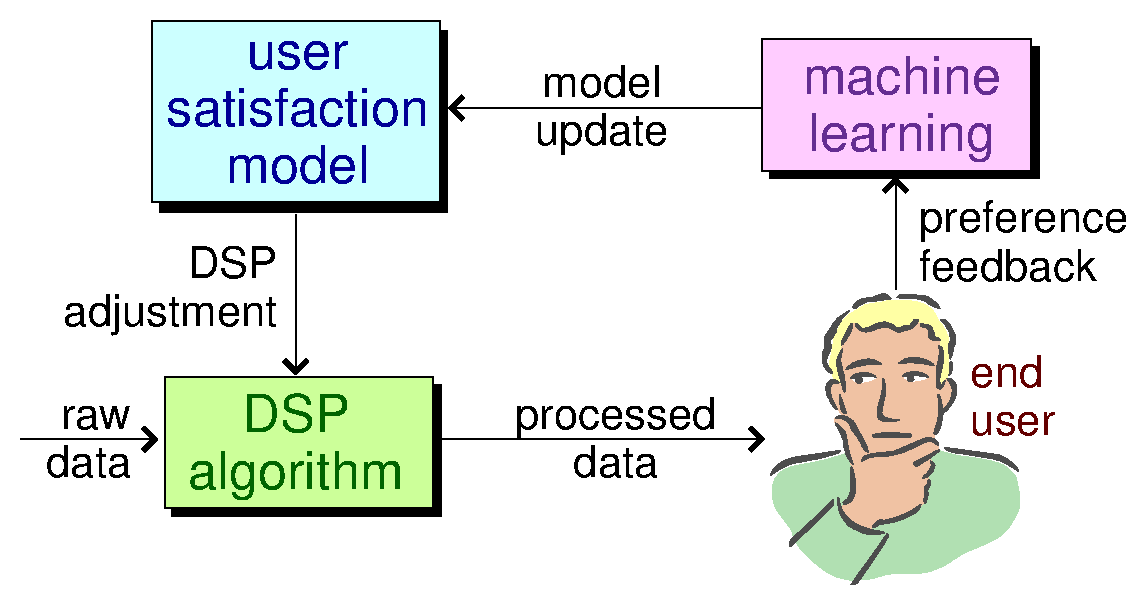
\includegraphics[width=8cm]{ML-SP-loop}
%%\caption{This is a figure.}
%\end{center}
%\end{figure}


Consider Figure~\ref{fig:ML-SP-loop} to illustrate my recent research work. A DSP algorithm transforms a raw input for presentation to an end user. In my current occupation, the DSP algorithm is a Hearing Aid (HA) processor and the end user a HA patient. As it is unknown which algorithm is optimal for the patient, we equip the DSP algorithm with adjustable parameters. Commercial HA algorithms contain about 140 of such tuning parameters (most of them under the hood). If we assume $5$ potentially interesting values for each parameter (e.g., very low, low, medium, large and very large), then the total number of parameter settings equals $5^{140}$, which is far more than the number of electrons in the universe (about $5^{115}$). Hence, the problem of finding the best HA algorithm for a patient is much like searching for a needle in a haystack.We cannot ask the patient to tune the DSP parameters himself, because the search space is too large and the preferred settings may change over time as the patient moves from his home into his car and later to an office environment.  
\begin{wrapfigure}{r}{0.5\textwidth}
  \vspace{-20pt}
  \begin{center}
    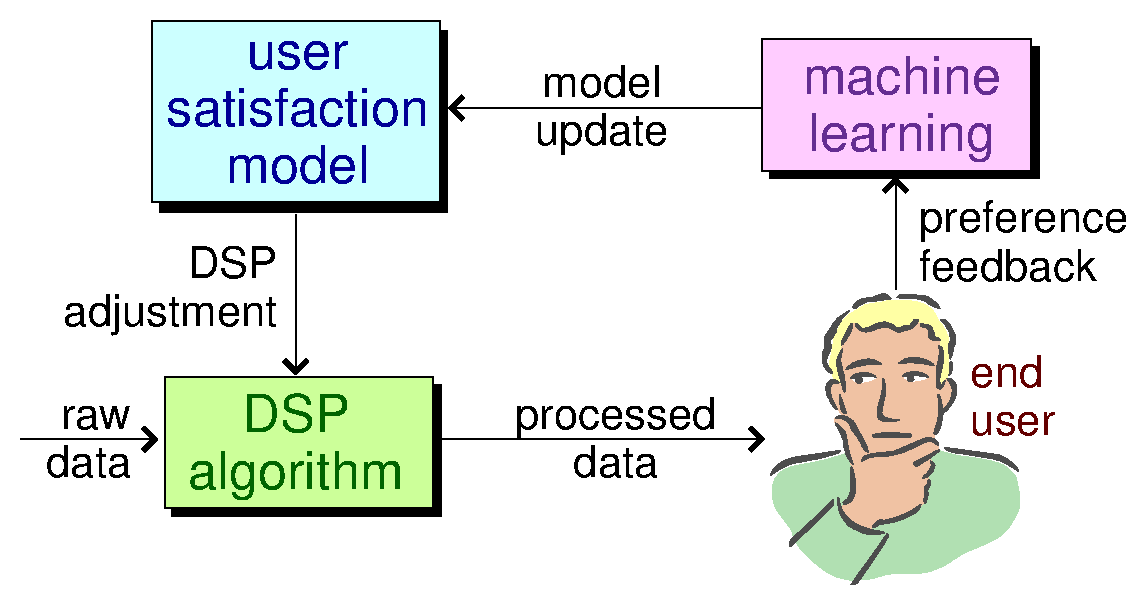
\includegraphics[width=0.48\textwidth]{ML-SP-loop}
  \end{center}
  \vspace{-20pt}
  \caption{Interactive machine learning for DSP personalization.}
  \vspace{-10pt}
  \label{fig:ML-SP-loop}
\end{wrapfigure}We can however ask the patient to provide the simplest form of preference feedback: just tab the HA (or shake his head, say a code word, etc.) if he's not happy with his HA processor. I created an interactive machine learning approach that learns the correct settings for the HA processor, straight from simple end user feedback and without loss of information. In principle, this approach extends to other applications areas such as customer personalization of TV monitors or tuning of medical image processing algorithms to maximize discovery of potentially malignant calcifications by a medical specialist. In general, signal processing and machine learning form complementary fields for the design of medical information processing systems with the end user in the loop.

\smallskip
At GN ReSound, I am a \textbf{Principal Scientist}. My DSP algorithms are integrated in many commercially available hearing aids, both for the Beltone and ReSound brand names. I am also affiliated as a \textbf{Research Fellow} with the Signal Processing Systems group (\url{w3.ele.tue.nl/en/sps}) at the Technical University Eindhoven (TU/e), where I teach a graduate class on adaptive information processing and supervise graduate students. Before ReSound, I was employed as a research scientist at Sarnoff Corporation (\url{www.sarnoff.com}) in Princeton, NJ, where I contributed to research projects over a wide range of signal and image processing topics such as word spotting, financial market prediction and breast cancer detection from mammograms. 
   
\vspace{-5mm} 
\subsubsection{(grant) writing}
\vspace{-5mm} 
As an research engineer, I design systems to solve problems. While a university researcher might justifiably attack problems that are `just' scientifically interesting, as an industrial researcher I seek to solve problems that are both interesting as well as commercially important. Throughout my research career, I've had a keen interest in linking scientific research to the real (commercial) world through writing of fund acquisition proposals (about 4 major successes), patents (about 13)  and scientific publications (about 60).  For example, through my affiliation with the TU/e, I wrote, together with Profs.\ Tom Heskes (RU Nijmegen) and Wouter Dreschler (VU Amsterdam), a research grant proposal (entitled: \emph{Personalization of Hearing Aids through Bayesian Preference Elicitation}), which in 2006 was awarded a 650 K\euro\ research grant by STW (Dutch government foundation for scientific research). At Sarnoff Corporation, I successfully acquired a 600K USD contract from an industrial client to develop speech processing algorithms for mobile telephones. 

\subsection{Management}\vspace{-5mm}
Over my career, I've managed research teams in both project and line managerial roles.  At ReSound, next to my role as a principal scientist, I am currently \textbf{head of the DSP Research group}, which encompasses about 10 researchers. Over the past 6 years, I've also served as ReSound's external research manager, which involves initiation, coordination and (budget) management of research projects that are executed in collaboration with top universities. Before ReSound, at Philips Hearing Systems  (1999-2000), I lead the algorithm R\&D group in developing DSP algorithms for the next generation of commercial hearing aids. Moreover, as an adjunct faculty member at the TU/e, I supervise graduate students and their research projects. 

\medskip
In general, my style of managing a high-quality engineering research group rests on three principles: (1) as a research leader, I strive to set and maintain a spot on the horizon for each project. Rather than working on a general area, I think that engineers are motivated by a challenge. Small successes are celebrated to keep the morale high. (2) Build a working system early, and iterate based on end user feedback. If the latter is not possible, still spend ample resources on testing to drive the direction of the project. (3) Finally, lead by example, since researchers are inspired by peers, not by managers. As a leader of a research group, I seek to set the example by partaking in the effort and filling holes where necessary. I've found that a sustained focus on these three principles improve the performance of both academic as well as industrial research projects.  

%\medskip
\subsection{Teaching} \vspace{-5mm}
Since 2004 I teach a core graduate-level class on adaptive information processing in the electrical engineering department at the Technical University Eindhoven (\url{http://www.sps.ele.tue.nl/members/b.vries/teaching/5mb20/index.html}). I have also organized several in-house courses at ReSound. I enjoy teaching and find it one of the more rewarding tasks that I work on. My teaching style derives from the philosophy that in order to really understand a concept, one must recreate it. In other words, learning involves creative activity from the student.  If the opportunity arises, I am prepared to develop courses in medical engineering, signal processing and machine learning at all academic levels. 


\newpage
\section{Curriculum Vitae}

\begin{llist}
\sectiontitle{\bf \b{Principal}\\ \b{Interests}}           
Signal processing, machine learning, computational neuroscience, biomedical engineering, research management, technical writing; applications to multimedia processing, medical devices, hearing rehabilitation and clinical trial design/analysis.  % information theory, VLSI for DSP
\sectiontitle{\bf \b{Academic} \\ \b{Background}}

\employer{{\bf 12/91, Ph.D. Electrical Engineering, \href{http://www.ece.ufl.edu/}{University of
Florida}}} \location{Gainesville, FL} Ph.D. research in signal
processing under direction of Professor Jose C. Principe.
Dissertation title: {\it Temporal processing with neural
networks---the development of the gamma model}.


\employer{{\bf 12/86, M.E. Electrical Engineering,
Technical University Eindhoven}} \location{Eindhoven, the
Netherlands} Focus areas: medical (thesis: intelligent alarms during anaesthesia) and
digital communications engineering.

\sectiontitle{\b{Employment} \\ \b{History}}

\employer{{\bf '12-pres., Professor, Eindhoven University of Technology, \href{http://www.sps.ele.tue.nl/}{Signal Processing Systems Group, EE dept.}}} \location{Eindhoven,
the Netherlands}
\vspace{-.8cm}
\begin{items}
  \item 1 day/week appointment; Previous engagement: Research Fellow ('04-'11)
  \item Research on \textbf{Personalization of Medical Signal Processing Systems}
  \item Teach graduate class on \href{http://www.sps.ele.tue.nl/members/b.vries/teaching/5mb20/index.html}{Adaptive Information Processing}.
  \item Inaugural lecture: "In Situ Personalization of Signal Processing Systems" (at \href{http://goo.gl/EoU0SE}{youtube}), September 2013. 
\end{items}


\employer{{\bf '99-pres., Principal Scientist, \href{http://www.gnresound.dk/}{GN ReSound} (Philips Hearing Technologies until 2001) }} \location{Eindhoven, the
Netherlands}
\vspace{-.8cm}
\begin{items}
  \item Other engagements include: DSP Functional Leader ('11-pres.), Head DSP Research ('08-'11), Manager External Research ('01-'08), Technology Leader ('99-'01, Philips)
  \item Research PI on low-power signal processing technology for the next
generation of digital hearing aids.
  \item Leadership/management tasks include(d) all aspects
of team and project management (teams of about 10 engineers); (responsible for) the corporate DSP research track, including the roadmap, budget and management; initiating and managing key studies at academic institutions and contract research organizations.
\end{items}




\employer{{\bf '93-'99, Member Technical Staff,  \href{http://www.sarnoff.com/}{Sarnoff
Corporation}}} \location{Princeton, NJ} 
\vspace{-.8cm}
\begin{items}
\item Research in advanced signal processing algorithms, initiating new technical and commercial thrusts, technical proposal writing and project management.
\item Principal investigator of funded projects on keyword spotting, digital hearing aids signal processing, speech enhancement and noise-robust speech recognition (co-PI). 
\item Co-initiated and developed signal processing in financial markets program at Sarnoff.
\item Member medical image processing research team. Funded projects include blind signal processing for breast mammography and perceptually optimized image coding.
\end{items}

\employer{{\bf '92-'93, Postdoctoral Fellow, David Sarnoff
Research Center}} \location{Princeton, NJ} 
\vspace{-.8cm}
\begin{items}
\item Developed neural
network based speech recognition method (50\% error reduction
relative to competing methods).
\end{items}

\employer{{\bf '87-'91, Research/Teaching Assistant,  University
of Florida}} \location{Gainesville, FL} 
\vspace{-.8cm}
\begin{items}
\item Taught and assisted in graduate classes in digital signal processing, control theory and computer architecture. 
\end{items}
\sectiontitle{\b{Special} \\ \b{Achievements}}

\employer{{\bf Awards}}
\begin{items}
\item Return-on-Performance Award, for technical work on
Speech Enhancement technology, Sarnoff Corporation, 1998
\item Achievement Award, for ''Leadership and technical contributions in
the area of adaptive speech enhancement'', Sarnoff Corporation, 1997
\item David Sarnoff Event Focus Award for ''Winning Sarnoff's First Commercial Contract for Speech Processing'', David Sarnoff Research Center, 1996.
\item Presidential Recognition Award, University of Florida, 1988.
\item $\delta$-Butterweck Award (awards top GPA), Technical University
Eindhoven, 1984.
\end{items}

\employer{{\bf Invited Lectures (selection)}}
\begin{items}
\item Leiden University Medical Center, keynote lecture on "Personalization of Medical Signal Processing Systems ", Leiden, January 2014 
\item Int'l Symposium on Auditory and Audiological Research (ISAAR), "Is Hearing Aid Signal Processing ready for Machine Learning", Nyborg (DK), August 2013
\item Clinical Physicist Post-graduate school, ''The Future of Hearing Aids'', Amersfoort January 2013
\item Delft Univ. of Technology, ''Machine Learning for Hearing Aids Technology'', Delft March 2012
\item International Forum for Hearing Instrument Developers, ''Bayesian Machine Learning for Hearing Aid Design, Fitting and Personalization'', Oldenburg (Germany), June 2011
\item University of Florida, ''Machine Learning Trends in the Hearing Aids Industry'', Gainesville, FL, April 2010 
\item SIKS Research School, ''Gaussian mixture models and the EM Algorithm'', Vught, Dec 2008
\item GN Nordic Audiology College, ''Learning technology in hearing aids'', Oslo, Norway, Sep 29, 2006
\item University of Nijmegen, ''Machine learning for hearing aids'', Nijmegen, Netherlands, June 2004
\item University of Florida, ''DSP for modern industrial hearing
aids'', Gainesville, FL, January 2004 
\item International Forum for Hearing Aid Developers ''Warped-frequency filterbanks'',
Oldenburg, Germany, July 2003 
\item Keynote address ''An
industrial perspective on intelligent hearing aids'' at 2nd
McMaster-Gennum Workshop on Intelligent Hearing Instruments, Niagara-on-the-Lake, ON, Sep 2001 
\item NIDCA/NASA/VA Hearing Aids Improvement Conference, May 1997 
\item Lucent Technologies, Bell Laboratories, November 1996 
\item AT\&T Research, July 1996 
\item NSA (U.S. Government), June 1993 
\item Neural Network Workshop, Rutgers University, October 1992 
\item David Sarnoff Research Center, October 1991
\end{items}

\employer{{\bf Professional Activities (selection)}}
\begin{items}
\item Associate Editor for \href{http://tnsre.bme.columbia.edu}{IEEE Transactions on Neural Systems and Rehabilitation Engineering}, 2012 - pres.
\item Invited member annual European Mathworks Advisory Board meetings, 2012 - pres.
\item Invited jury member for Open Technology Program (OTP) research proposals to Dutch Technology Foundation STW, Dec. 2010
\item Invited DSP expert on IWT (Flemish Institute for Science and Technology) panel to evaluate candidate PhD proposals, Brussels, Nov. 2005 and May 2006
\item Organizer/chair special session `DSP for Intelligent Hearing Aids', ICASSP 2002,
Orlando, FL, May 2002
\item Publicity chair, Neural Networks for Signal Processing Workshop,
Amelia island, Florida, 1997 and Cambridge, UK, 1998
\item Session chair Non-linear Systems Identification, ICASSP96,
Atlanta, GA, May 1996, and IEEE NNSP-98 Workshop, Cambridge, UK,
September 1998
\item (Elected) member of ''IEEE Technical Committee on Neural Networks for Signal Processing Society'', 1995-1998
\item Invited researcher in government sponsored Robust Speech Processing Workshop, July-August 1993
\item Member of various professional societies (e.g. IEEE, INNS)
\end{items}


\employer{{\bf Refereed Publications}}

IEEE Transactions on Signal Processing, IEEE Transactions on
Neural Networks, NeuroComputing Journal, Neural Networks Journal,
EURASIP Journal of Applied Signal Processing, Advances in Neural
Information Processing Systems (NIPS) Conferences, ICASSP
Conferences and others.
\sectiontitle{\b{TU/e Univ.} \\ \b{Activities}}
\employer{{\bf Teaching}}
\begin{items}
\item \href{http://www.sps.ele.tue.nl/members/b.vries/teaching/5mb20/home.html}{\textbf{Adaptive Information Processing}}. Together with \href{http://www.sps.ele.tue.nl/members/T.J.Tjalkens}{Tjalling Tjalkens}, since spring 2005 I teach a core graduate class on the fundamentals of machine learning.
\item \href{http://www.sps.ele.tue.nl/members/b.vries/teaching/mlrc04/home.html}{\textbf{Machine Learning}}. I organized a machine learning reading club for TU/e graduate students and GN ReSound staff. Fall 2004.
\end{items}

\employer{{\bf Research}}

My current research focuses on applications of Bayesian machine learning to personalization of hearing aid algorithms. In July 2006, together with  \href{http://www.cs.ru.nl/staff/Tom.Heskes}{Tom Heskes} and \href{http://www.ac-amc.nl/medewerkers/dreschler.html}{Wouter Dreschler}, we received a $650$K euro grant from \href{http://www.stw.nl}{STW} to pursue further research on \emph{Personalization of Hearing Aids through Bayesian Preference Elicitation}.

\employer{{\bf Recent Student Supervision}}
\begin{items}
\item Brian Hutama Susilo, M.Sc. practical training project, \emph{Automated Tuning Algorithm for Low-latency PC-based Audio Processing}, Dec. 2013
\item Zijian Xu, M.Sc. thesis project, \emph{Fast Design of Audio Processing Algorithms by Interactive Parameter Exploration}, August 2013
\item Timur Bagautdinov, M.Sc. thesis project, \emph{A Machine Learning Framework for Signal Processing}, August 2013 
\item Marno van der Maas, B.Sc. research project, \emph{Browser-based Remote Control of Hearing Aids}, June 2013
\item Maarten Thomassen, M.Sc. practical training project, \emph{Spectral Audio Monitoring}, July 2012
\item Joris Kraak, M.Sc.-thesis, \emph{Computer-Aided Algorithm Design for Audio Processing}, April 2012
\item Joris Kraak, M.Sc. practical training project, \emph{Optimization of a Spectral 
Noise Tracking Algorithm}, Dec. 2010
\item Jianfeng Li, M.Sc.-thesis, \emph{Acoustic scene-adaptive speech enhancement}, Aug. 2010
\item Jianfeng Li, M.Sc.-project, \emph{Spatial defect clustering on semiconductor wafers using image processing techniques}, Aug.-2009
\item Xueru Zhang, P.D.Eng.-thesis: \emph{Bayesian periodogram smoothing for speech enhancement}, Sep. 2008
\item Rene Besseling, M.Sc.-project, \emph{Gaussian processes in Bekesy audiometry}, June 2008
\item Serkan Ozer, M.Sc.-thesis: \emph{Bayesian linear regression for user-adaptive hearing aids}, Aug. 2007
\item Ronnie van Loon, M.Sc.-thesis: \emph{a Probabilistic Approach to Sound Classification}, June 2007.
\item Anton Vakrushev, P.D.Eng.-thesis: \emph{Interactive machine learning for Personalization of hearing aid algorithms}, Sep. 2006
\item Jorik Caljouw, M.Sc. practical training on \emph{PDA-based Interfacing to a real-time audio platform}, Dec. 2005.
\item Paul Aelen, M.Sc. project, \emph{Determination of the Intra Uterine Pressure with electrodes on the abdomen}, Dec. 2005.
\item Job Geurts, M.Sc. practical training on \emph{A PC-based real-time simulation platform for evaluating hearing aid algorithms}, Jun. 2005.
\end{items}


\employer{{\bf Care and Cure theme}}

I actively participated in the development of the Care and Cure theme roadmap for the EE department (2008).  
\sectiontitle{\b{Personal}}
Born on June 28th 1962. Dutch citizen. Leisure interests: sports, travel and reading.

\sectiontitle{\b{References}}
\href{http://www.cnel.ufl.edu/principe/principe.html}{Dr. Jose C. Principe}, Distinguished Professor of Electrical Engineering, (Ph.D. supervisor).\\
University of Florida, Gainesville, FL \\
e-mail \texttt{principe@synapse.ee.ufl.edu}

% \par
% \href{http://liinc.bme.columbia.edu/liinc_people_sajda.htm}{Dr. Paul Sajda}, Associate Professor of Biomedical Engineering. \\
% Columbia University, 1013 CEPSR-Schapiro Center, mc8904 530 W.
% 120th Street New York, NY 10027 \\
% e-mail \texttt{ps629@columbia.edu}

\par
Other references on request.

%\newpage
\sectiontitle{\b{Publications}}

\employer{{\bf Impact Factor}}
\begin{itemize}
\item 10 journal articles, 13 patents, $>$50 conference contributions with  citation numbers (high to low) $\r{146,108,69,33,33,31,30,29,21,16,14,12},11,11,10,7,7,\ldots \Rightarrow$ Hirsch-index $= 12$, Google Scholar, Feb-2011.
\item ($>$60 unpublished technical reports (company confidential))
\end{itemize}


\employer{{\bf Journal Articles and Book Chapters}}

%\renewcommand{\refname}{\vspace{-1.5cm}}
\begin{etaremune}

\item Rik Vullings et al.\, An Adaptive Kalman Filter for ECG Signal Enhancement, \emph{IEEE Transactions on Biomedical Engineering}, vol.58, no.4, April 2011.

%\item \gray{Bert de Vries et al., Evidence-based design of hearing aid algorithms, submitted to \emph{J. acoustic soc. of America}, Jan.\ 2008.}

\item A.\ Ypma et al., \href{http://www.hindawi.com/GetArticle.aspx?doi=10.1155/2008/183456}{On-line Personalization of Hearing Instruments}, \emph{EURASIP Journal on Audio, Speech, and Music Processing}, September 2008.

\item  Tjeerd Dijkstra et al., \href{http://www.hearingreview.com/issues/articles/2007-10_05.asp}{The Learning Hearing Aid: Common-Sense Reasoning in Hearing Aid Circuits}, The Hearing Review, issue October 2007. (cited by 5, GS1102 (=Google Scholar, 2011-02))

%\item \gray{Thomas Beierholm et al., Non-Stationary Noise Reduction by Particle Filtering in a Cascade Formant Synthesizer Model, submitted to \emph{IEEE Trans. on Audio, Speech and Language Processing}, June 2007}

\item David Zhao et al., On-line Noise Estimation Using Stochastic-Gain HMM for Speech Enhancement, \emph{IEEE Transactions on Audio, Speech and Language Processing}, vol.16, no.4, May 2008. (cited by 2, GS0808)

\item Jose Principe et al., Locally Recurrent Networks: The Gamma
Operator, Properties and Extensions, invited book chapter in {\em
Neural Networks and Pattern Recognition}, Omidvar and Dayhoff
(eds.), Academic Press, 1997. (cited by 1, GS0907)

\item Bert de Vries, Short term memory structures for dynamic neural networks, book chapter in:
{\em Artificial Neural Networks for Speech and Vision}, Richard Mammone (ed.), Chapman \& Hall Ltd.,
1994. (cited by 3, GS0810)

\item Bert de Vries and Jose Principe, The gamma model--A new neural
network for temporal processing, {\em Neural Networks} vol. 5(4),
pp. 565-576, 1992. \r{(cited by 146, GS1102)}

\item Jose Principe and Bert de Vries, The gamma filter--A new class of adaptive IIR filters
with restricted feedback,  {\em IEEE transactions on signal
processing}  vol. 41(2), pp. 649-656, 1992. \r{(cited by 108, GS1102)}

\item Bert de Vries, \href{http://ufdc.ufl.edu/UF00082173/00001}{Temporal processing with neural networks-the development of the Gamma model},
{\em Ph.D. dissertation}, University of Florida, 1991. \r{(cited by 12, GS1102)}

\item Joachim Gravenstein et
al., Sampling intervals for clinical monitoring of variables during
anesthesia,  {\em Journal of clinical monitoring} vol 5(1), 1989. \r{(cited by 30, GS1102)}

\item Jan J. van der Aa, Bert de Vries and Joachim
Gravenstein, Toward more sophisticated monitoring alarms,  {\em
Journal of clinical monitoring} 4 (2), 1986.

\end{etaremune}
 

%\newpage
\employer{{\bf Patents}}

\begin{etaremune}

\item Andrew Dittberner et al., A Location Learning Hearing Aid, filed by GN ReSound with Danish Patent and Trademark Office, December 2013

\item Bert de Vries and Mojtaba Farmani, A Hearing Aid with Probabilistic Hearing Loss Compensation, filed by GN ReSound with US Patent and Trademark Office, App. number 14077031, Nov. 2013 

\item Bert de Vries et al., Efficient evaluation of hearing ability, submitted by GNR Ref.: P1669 EP, Albihns Ref.: P13304 US / P13303, April 2009.

\item Alexander Ypma et al., Asymmetric synchronization of hearing aid algorithms, submitted by GN ReSound, patent no. 09174982.0-2225, filed 4-Nov-2009.

\item Alexander Ypma et al., Learning control of hearing aid parameter settings, submitted by GN ReSound, filed 16-Mar-2007.

\item Bert de Vries and Alexander Ypma, Optimization of Hearing Aid Parameters, filed by GN ReSound, patent no. WO/2007/042043, 10/13/06.

\item Bert de Vries, Bastiaan Kleijn, Alexander Ypma and David Zhao, Method and Apparatus for Improved Estimation of Non-stationary Noise for Speech Enhancement, filed by GN ReSound, patent no. 06119399.1-224, 08/23/06

\item Bert de Vries and Rob de Vries, Fitting methodology and hearing prosthesis based on signal-to-noise ratio loss data, USA patent registered for
GN ReSound, no. 20040047474, 03/11/2004.

\item L. Parra and B. de Vries, Method and apparatus for adaptive speech detection by applying a probabilistic description to the classification and tracking of signal components, patent registered for Sarnoff Corporation, LG Electronics, Inc., no. 6691087, 10-Feb. 2004. (cited by 3, GS1102)

\item Bert de Vries, Noise Spectrum Tracking for Speech Enhancement,
patent registered for Sarnoff Corporation, no. US6289309,
9/11/2001. \r{(cited by 29, GS1102)}

\item  J. Lubin et al., Method and apparatus for training a neural network to learn and use fidelity metric as a control mechanism, patent registered for
Sarnoff Corporation, no. US6075884, 6/13/2000. \r{(cited by 14, GS1102)}

\item Bert de Vries, Method and apparatus for filtering signals using a gamma delay line based estimation of power spectrum, patent
registered for Sarnoff Corporation, no. US6073152, 6/6/2000. (cited by 1, GS1102)

\item M. Brill, J. Lubin, B. de Vries, O. Finard, Method and apparatus for assessing the visibility of differences between two image sequences, patent registered for Sarnoff Corporation, no.
US5974159, 10/26/1999. \r{(cited by 33, GS1102)}

\item Bert de Vries, Method and system for training a neural network with adaptive
weight updating and adaptive pruning in principal components space,
patent registered for David Sarnoff Research
Center, no. 5,812,992, 9/22/98. \r{(cited by 21, GS1102)}

\item Bert de Vries and Jose Principe, An adaptive filter based on a recursive delay line,  patent registered
for University of Florida, no. 5,301,135, April 1994. (cited by 5, GS1102)

\end{etaremune}

% \employer{{\bf Sarnoff Technical Reports}}

% \begin{etaremune}

% \item Bert de Vries, Uday Jain, Lucas Parra, Low-complexity spectrum
% based speech enhancement, \emph{Sarnoff Technical Report}, March
% 1998.

% \item Bert de Vries, Finding dependencies in foreign exchange rate data
% by the delta test, \emph{Sarnoff Technical Report}, December 1995.

% \item Bert de Vries, Adaptive prediction with error bars and an
% application to foreign currency trading, \emph{Sarnoff Technical
% Report}, July 1995.

% \item Bert de Vries, Adaptive eigenpruning for non-stationary time
% series modeling with applications to foreign exchange rate
% forecasting, \emph{Sarnoff Technical Report}, October 1994.

% \end{etaremune}

\employer{{\bf Conferences and Workshops}}
\begin{etaremune}

\item Bert de Vries and Andrew Dittberner, Is Hearing Aid Signal Processing Ready for Machine Learning? \emph{Int'l Symposium on Auditory and Audiological Research}, Nyborg, DK, Aug. 2013

\item Ungureanu C. et al., A Bayesian Network for Detection of Seizures, \emph{1st Jan Beneken Conference on Modeling and Simulation of Human Physiology}, Eindhoven, NL, 2013

\item Petkov P. et al., Discrete Choice Models for Non-Intrusive Quality Assessment, \emph{Interspeech 2011}, Florence, Italy, 2011

\item Rob de Vries et al., A software suite for automatic beamforming calibration, \emph{Int'l Hearing Aid Research Conference}, Lake Tahoe, CA, August 2010

\item S.I. Mossavat et al., A Bayesian hierarchical mixture of experts approach to estimate speech quality, \emph{QoMEX 2010},  Trondheim, Norway, June 2010

\item Jos Leenen and Bert de Vries, Current DSP and Machine Learning Trends in the Hearing Aids Industry,  \emph{IEEE Benelux Signal Processing Symposium: Signal Processing for Digital Hearing Aids}, Delft, NL, April 2010

\item Xueru Zhang et al., Bayesian periodogram smoothing for speech enhancement, \emph{European Symposium on Artificial Neural Networks (ESANN-09)}, Bruges, April 2009

\item Adriana Birlutiu et al., Towards hearing aid personalization: preference elicitation from audiological data, \emph{Scientific ICT-Research Event Netherlands (SIREN)}, Amsterdam, Sep. 2008

\item Tjeerd Dijkstra et al., HearClip: an Application of Bayesian Machine Learning to Personalization of Hearing Aids, Presentation at \emph{Dutch Society for Audiology Meeting}, Sep. 2008

\item Bert de Vries, Fast Model-Based Fitting through Active Data Selection, \emph{Int'l Hearing Aid Research Conference}, Lake Tahoe, CA, August 2008

\item Rolph Houben et al., Construction of a virtual subject response database to reduce subject testing, \emph{Int'l Hearing Aid Research Conference}, Lake Tahoe, CA, August 2008

\item Bert de Vries et al., The Complexity of Hearing Aid Fitting, presented at \emph{International Symposium on Auditory and Audiological Research 2007}, Helsingor, Denmark, August 2007

\item Jos Leenen et al., Learning Volume Control for Hearing Aids, presented at \emph{International Symposium on Auditory and Audiological Research 2007}, Helsingor, Denmark, August 2007

\item Alexander Ypma et al., Bayesian Feature Selection for Hearing Aid Personalization,  \emph{MLSP-07}, Thessaloniki, Greece, 2007. (cited by 2, GS1102)

\item Adriana Birlutiu et al., Personalization of Hearing Aids through Bayesian Preference Elicitation, \emph{NIPS workshop on User Adaptive Systems}, Whistler, BC, Canada, December 2006

\item Bert de Vries et al., Bayesian Machine Learning for Personalization of Hearing Aid Algorithms, \emph{Int'l Hearing Aid Research Conference}, Lake Tahoe, CA, August 2006

\item Alexander Ypma, Bert de Vries and Job Geurts, Robust Volume Control Personalization from On-line Preference Feedback, \emph{IEEE Int. Workshop on
Machine Learning for Signal Processing}, Maynooth, Ireland, 2006. (cited by 4, GS1102)

\item Bert de Vries, Tom M. Heskes and Tjeerd M. H. Dijkstra, Bayesian Incremental Utility Elicitation with Application to Hearing Aids Personalization, \emph{Valencia/ISBA 8th World Meeting on Bayesian Statistics}, Benidorm, Spain, June 2006

\item Tjeerd M. H. Dijkstra et al., A Bayesian decision-theoretic framework for psychophysics, \emph{Valencia/ISBA 8th World Meeting on Bayesian Statistics}, Benidorm, Spain, June 2006

\item Alexander Ypma, Bert de Vries and Job Geurts, A learning volume control that is robust to user inconsistency,  \emph{The second annual
IEEE BENELUX/DSP Valley Signal Processing Symposium}, Antwerp, March 2006

\item Paul Aelen et al., Electrohysterographic Estimation of the Intra-Uterine Pressure, \emph{The second annual
IEEE BENELUX/DSP Valley Signal Processing Symposium}, Antwerp, March 2006

\item Tom Heskes and Bert de Vries, Incremental Utility Elicitation for Adaptive
Personalization, \emph{The 17th Belgian-Dutch Conference on Artificial Intelligence}, Brussels, Belgium, October 2005. (cited by 6, GS1102)

\item Bert de Vries and Rob de Vries, An Integrated Approach to Hearing Aid Algorithm Design, \emph{Int'l Hearing Aid Research Conference},
Lake Tahoe, CA, August 2004

\item Harald Pobloth et al., Speech Coding for Wireless Communication
in the Hearing Aid Environment, \emph{Int'l Hearing Aid Research Conference},
Lake Tahoe, CA, August 2004

\item Bert de Vries and Rob de Vries,An Integrated Approach to Hearing
Aid Algorithm Design for Enhancement of Audibilit y,
Intelligibility and Comfort, \emph{IEEE Benelux Signal Processing
Symposium}, Hilvarenbeek, Netherlands, April 2004. (cited by 4, GS1102)

\item Rob de Vries and Bert de Vries, Toward SNR-Loss Restoration in Digital Hearing Aids, {\em ICASSP 2002}, Orlando, FL, May 2002. (cited by 4, GS0801)

\item Bert de Vries, Jos Leenen, A Low Power Digital AGC Circuit for
Dynamic Range Control of an A/D Converter, {\em International
Hearing Aids Research (IHCON) Conference 2000}, Lake Tahoe (CA),
August 2000

%Bert de Vries, Improved Noise Spectrum Tracking for Speech
%Enhancement, submitted to {\em ICASSP'99}
%\item

\item Lucas Parra, Clay Spence and Bert de Vries, Convolutive Blind Source
Separation based on Multiple Decorrelation, {\em IEEE workshop on Neural
Networks for Signal Processing VIII}, pp.23-32, Cambridge, UK, 1998. \r{(cited by 69, GS1102)}

\item Bert de Vries, Blind Signal Processing for Hearing Aids, {\em NIH Hearing Aids Improvement Conference}, Bethesda, MA, May 1997

\item Bert de Vries, Adaptive Gamma Filters for Miniature Hearing Aids, {\em NIH Hearing Aids Improvement Conference},
Bethesda, MA, May 1997

\item Bert de Vries, Adaptive rank filtering based on error minimization,
{\em ICASSP-97}, Munich, April 1997

\item Lucas Parra, Clay Spence, Bert De Vries, Convolutive Source Separation
and Signal Modeling with Maximum Likelihood, {\em International
Symposium on Intelligent Systems} (ISIS'97), 1997, Regio Calabria,
Italy. \r{(cited by 10, GS1101)}

\item Q. Lin et al., Robust distant-talking speech recognition,  {\em
ICASSP-96}, Atlanta,GA, May 1996. \r{(cited by 16, GS1102)}

\item Bert de Vries et al., Neural network speech enhancement for noise robust speech recognition,
{\em International Workshop on Applications of Neural Networks to Telecommunications}, Sweden, May
1995. (cited by 2, GS1102)

\item Lin et al., Experiments on distant-talking speech recognition, {\em ARPA Workshop on Spoken
Language Technology}, Austin, TX, January 1995.\r{(cited by11, GS1102)}

\item Qiguang Lin et al., System of microphone arrays and neural networks for robust speech recognition in multimedia
environments, Proceedings {\em International Conference on Spoken Language
Processing}, Yokohama, Japan, September 1994. (cited by 8, GS1102)

\item Bert de Vries, Gradient-based adaptation of network structure, {\em International Conference on
Artificial Neural Networks 94}, Sorrento, Italy, May 94.

\item Che et al., Microphone Arrays and Neural Networks for Robust Speech
Recognition, {\em ARPA
Workshop on Human Language Technology}, Princeton, NJ, March 1994.\r{(cited by 33, GS1102)}

\item Bert de Vries et al., An application of Gamma delay lines to "BDG" phoneme classification,
{\em Government Microcircuit Applications Conference proceedings}, New
Orleans, LA, November 1993.

\item Bert de Vries, Time-varying neural networks for large tasks, {\em International Conference on Artificial
Neural Networks proceedings}, Amsterdam, the Netherlands, September
13-16, 1993.

\item  J.C. Principe et al., Backpropagation through time with fixed memory size requirements, \emph{Proceedings of Workshop on Neural Networks for Signal Processing}, Linthicum Heights, MD, USA, Sep. 1993. (cited by 1, GS1102)

\item Bert de Vries et al.,Learning with target trajectory constraints for sequence classification tasks,
{\em ICASSP-93}, Minneapolis, MN, April 1993.

\item Bert de Vries et al.,Short Term Memory Structures for Dynamic Neural
Networks,  {\em Asilomar-92}
Conference proceedings, Pacific Grove, CA, 1992. (cited by 3, GS1102)

\item T. Oliveira a Silva et al., Generalized feedforward filters with
complex poles, {\em Proceedings of the
1992 IEEE workshop on Neural Networks for Signal Processing},
Copenhagen, Denmark, 1992.

\item Jyh-Ming Kuo, Jose Principe and Bert de
Vries, Prediction of chaotic time series using recurrent networks,
{\em Proc. of the 1992 IEEE workshop on Neural Networks for Signal
Processing}, 1992. \r{(cited by 7, GS1102)}

\item Jose Principe, Bert de Vries and
Pedro G. de Oliveira, Generalized feedforward structures: a new class
of adaptive filters, {\em ICASSP-92}, San Francisco, vol. IV,
pp. 245-248, 1992. \r{(cited by 7, GS0801)}

\item T. Oliveira e Silva, P. Guedes de Oliveira, J. C. Principe and B.
de Vries, A Complex Pole Extension to the Gamma Filter, {\em The
INESC Journal of Research and Development}, vol. 3, no. 1, pp.
35-41, Jan./Jun. 1992.

\item Bert de Vries et al., Adaline with adaptive recursive memory, {\em Proceedings IEEE workshop on signal
processing}, Princeton, NJ, 1991. \r{(cited by 11, GS1102)}

\item Principe et al., Modeling applications with the focused gamma
net,  {\em NIPS-4 proceedings},
Denver, CO, 1992. \r{(cited by 6, GS0810)}

\item Bert de Vries et al., Some practical issues concerning the gamma
neural net, {\em Proceedings IJCNN-91},
Seattle, WA, 1991.

\item Bert de Vries and Jose Principe, A theory for neural nets with time
delays, {\em NIPS-3 Proceedings},
Denver, 1991. \r{(cited by 31, GS1102)}

\item Bert de Vries et al., Neural net models for temporal processing, {\em Proceedings nineth southern biom. eng. conference}, Miami, FL, 1991.

\item Bert de Vries et al., A new neural net model for temporal processing,
{\em 12th ann. int. conf. IEEE on
the eng. in medicine and biology society}, Philadelphia, PA, 1990.

\item Bert de Vries et al., Artificial neural networks as a computational paradigm for detection of anaesthetic complications,
{\em Computers in Anesthesia 10}, New Orleans, LA, 1989.

\item Bert de Vries et al., Distribution of anesthesia related occurrences during surgical operations,
{\em Anesthesiology review} 14 (6), 1987.

\end{etaremune}


\end{llist}
\end{document}
